\subsubsection{\textit{EL} script}

\par The listing \ref{lst:EL_Gen} corresponds to the implementation of the component \texttt{Generator}. Line 1 and 2 include the necessary files to use the language and the interfaces definition. The component \texttt{Generator} has two properties. The default value of the property \texttt{optimizations} is \texttt{false} and this means that the code optimizations will not run it the configuration file value is leaved by default. The property \texttt{trgCodeTracing} is set to \texttt{true} by default, this means that the translated instructions will be printed in serial port console at execution.
\par The service \texttt{s\_Generate} is declared at line 10. The references' declaration starts at line 11.

\begin{lstlisting}[language=EL, caption=Generator (EL representation)., label=lst:EL_Gen]
	import "Languages.el"
	import "Interfaces.el"
	
	component Generator (C)
	{
		properties:
		bool optimizations : false
		bool trgCodeTracing : true
		services:
		i_Generate s_Generate	
		references:
		i_Registers r_SrcRegisters
		i_Registers r_TrgRegisters
		i_SrcEnv r_SrcEnv
		i_ISA r_ISA
		i_TCache r_TCache
		i_DMem r_DMem				
		i_EngineState r_EngineState
	}
\end{lstlisting}

\subsubsection{Elaborations}

After all the EL scripts are made with all component, properties, interfaces and the binds, the next step is compile the DBT. To make this it is only necessary to click with right button of the mouse above the script with the top level, as is shown in the figure \ref{fig:compileel}.

\begin{figure} [H]
	\centering
	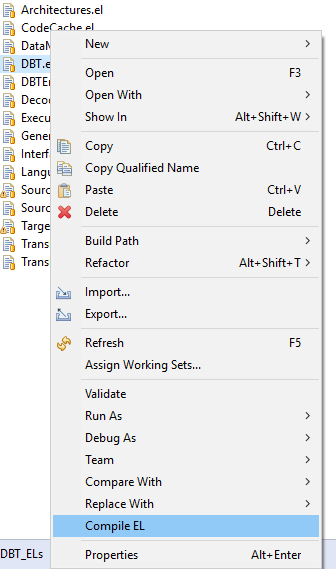
\includegraphics[width=0.4\linewidth]{Images/compileEL}
	\caption{Compile EL scripts}
	\label{fig:compileel}
\end{figure}

This will generate a series of files Java and XML (listing \ref{lst:genXML}). The two most important directories are the \texttt{Configs} where the configurable XML is stored and the \texttt{SpecificElaborations} where it generates a template for each component. 
If the template change is not desired, and because when the EL is compiled the file is overwritten, the XML of a specific component should be altered to have the specific elaboration file that is wanted.
In the case of the \texttt{Generator} it is wanted the \texttt{SpecificGeneratorElaborator} instead of template that is set by default so the XML is altered as shown in the line  of the following XML.
\begin{lstlisting}[language=XML, caption=Generator XML., label=lst:genXML]
	<component type="Generator">
		<elaboration default="SpecificGeneratorElaboratorTemplate">SpecificGeneratorElaborator</elaboration>
		<properties>
			<property type="bool" name="optimizations" default="false">
				<value>
					<element>true</element>
				</value>
			</property>
		</properties>
	</component>
\end{lstlisting}

The source files of DBT with annotations should be placed in the same folder of the specific elaboration for the component that models that code, or in the folder shared sources if the source as annotations that refer to different components. 

The annotations that the elaborator for the generator replaced are described in table \ref{annotationTable}.
\begin{table}[h]
	\caption{Code generation functions.}
	\label{annotationTable}
	\centering
	\begin{tabular}{|l||l||l|}
		\hline
		\textbf{Annotations} 	& \textbf{File} 			& \textbf{Type}\\ \hline
		Generator\_optimization & TargetArch\_CortexM3.h 	& Property replacement \\ \hline
		Generator\_cacheCode	& TargetArch\_CortexM3.cpp	& Interface Functions replacement \\ \hline
		Generator\_getPC		& TargetArch\_CortexM3.cpp	& Interface Functions replacement \\ \hline
		Generator\_readDataMem	& TargetArch\_CortexM3.cpp	& Interface Functions replacement \\ \hline
		Generator\_eoBB			& TargetArch\_CortexM3.cpp	& Interface Functions replacement \\ \hline
		Generator\_eoExec		& TargetArch\_CortexM3.cpp	& Interface Functions replacement \\ \hline
		Generator\_tracing		& SharedSources/types.h		& String replacement \\ \hline
		
	\end{tabular}
\end{table}	

The table shows that the generator is only going to alter the files TargetArch\_CortexM3.h and TargetArch\_CortexM3.cpp and a shared source named types.

The third column of the table as the type of replacement. As it is possible to observe there are three types the first one is replace the annotation with the value of a property that is altered in the XML file. 

The second type is the interface functions replacement to respect the interfaces from the model. If a component makes reference to a service in component, the user needs to alter the code and replace a annotation, that is according with the function of that interface, in order to respect the reference architecture. 

And last type is a direct string replacement. In this case it is used a property to know if the elaborator should comment or simply delete the annotation. The elaborator replace with a string with the comment or with nothing, deleting the annotation from the source file.

The process to make the specific elaborator for a component, is to use the AbstractElaborator API to open sources and replace their annotations. Listing \ref{lst:genElab} is the specific elaboration file of generator with the strings that should substitute the annotations. 

\begin{lstlisting}[language=Java, caption=Generator Specific Elaborator., label=lst:genElab]
package EL.SpecificElaborations.Generator.SpecificGeneratorElaborator;  

import EL.Components._Generator;
import EL.Elaborations.AbstractGeneratorElaborator;
import EL.ElaborationError;
import java.util.ArrayList;
import EL.ConfigReader.SpecificConfigReader;
import EL.Elaborations.*;
import EL.ConfigReader.*;
import EL.Components.*;

public class SpecificGeneratorElaborator extends AbstractGeneratorElaborator {
	SpecificConfigReader scr = null;

	public void generate(){
		System.out.println("This is the Generator template specific elaboration.");
		openAnnotatedSource("TargetArch_CortexM3.h");
		replaceAnotation("Generator_optimization",String.valueOf(target.get_optimizations()));

		openAnnotatedSource("TargetArch_CortexM3.cpp");		
		AbstractTranslationCacheElaborator TCacheElab = (AbstractTranslationCacheElaborator) getElaborator((_TranslationCache) target.get_r_TCache());
		replaceAnotation("Generator_cacheCode", (String) TCacheElab.getI_TCacheElaboratorCacheCode());

		AbstractSourceEnvElaborator SrcEnvElab = (AbstractSourceEnvElaborator) getElaborator((_SourceEnv) target.get_r_SrcEnv());
		replaceAnotation("Generator_getPC", (String) SrcEnvElab.getI_SrcEnvElaboratorGetPC());

		AbstractDataMemoryElaborator DataMemElab = (AbstractDataMemoryElaborator) getElaborator((_DataMemory) target.get_r_DMem());
		replaceAnotation("Generator_readDataMem", (String) DataMemElab.getI_DMemElaboratorReadDataMem());

		AbstractDBTEngineElaborator DBTEngineElab = (AbstractDBTEngineElaborator) getElaborator((_DBTEngine) target.get_r_EngineState());		

		replaceAnotation("Generator_eoBB", (String) DBTEngineElab.getI_EngineStateElaboratorEoBB());
		replaceAnotation("Generator_eoExec", (String) DBTEngineElab.getI_EngineStateElaboratorEoExec());

		openAnnotatedSharedSource("types.h");
		if(target.get_trgCodeTracing()==false)
			replaceAnotation("Generator_tracing","//");
		else
			replaceAnotation("Generator_tracing","");
	}
\end{lstlisting}